Tras establecer los parámetros correspondientes a la gestión del proyecto, este capítulo presenta el diseño del sistema desarrollado. Para ello se aborda: el diseño de agentes basado en LangGraph, la arquitectura distribuida del sistema multiagente, la implementación de servidores y cliente MCP, y la estructura de directorios del proyecto.

\section{Diseño de agentes}
LangGraph proporciona un marco de trabajo estructurado para la creación de flujos de ejecución en forma de grafo. Estos grafos se construyen mediante el objeto \opus{StateGraph} para establecer la lógica de enrutamiento entre nodos, lo que requiere un estado compartido que coordine la ejecución. Los nodos se definen como funciones de Python que operan sobre el estado del grafo, representado por un diccionario tipado. El sistema permite dos tipos de nodos: los de ejecución realizan operaciones modificando el estado, mientras que los condicionales determinan qué nodo ejecutar según el estado actual.

La Figura \ref{fig:react} ejemplifica este paradigma mediante una implementación del patrón ReAct (véase Sección \ref{sec:react}). La ejecución se inicia en el nodo de razonamiento, donde una función invoca al LLM y almacena la respuesta como mensaje en el estado. Posteriormente, el nodo condicional \opus{should_continue()} evalúa si la respuesta del modelo requiere iteraciones adicionales: cuando contiene llamadas a herramientas se procede a ejecutarlas, mientras que su ausencia indica que la consulta ha sido resuelta. Tras la ejecución de las herramientas, se incorpora su resultado a los mensajes del estado, reiniciando el paso de razonamiento con la nueva información.

\begin{figure}[hbtp]
  \centering
  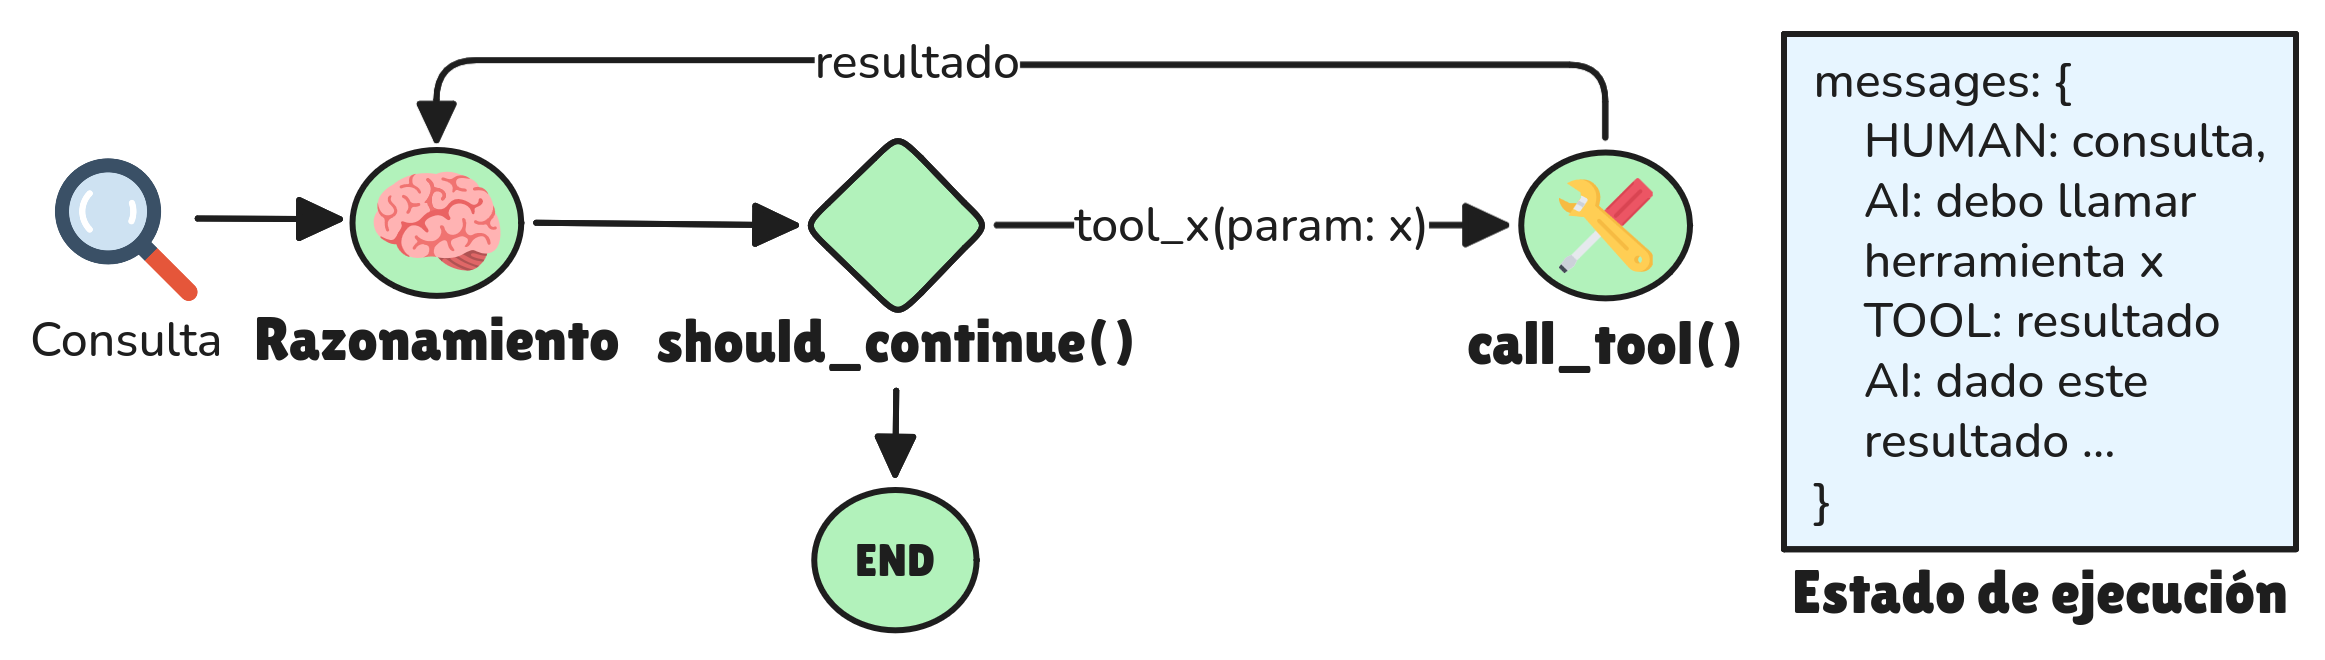
\includegraphics[scale=0.2]{figures/react.png}
  \caption{Esquema de implementación de patrón ReAct en Langgraph}
  \label{fig:react}
\end{figure}

Este enfoque proporciona un marco de trabajo orientado a la composición, donde un nodo puede constituir a su vez otro grafo compilado que represente a otro agente. No obstante, surge el problema de redundancia cuando dos agentes comparten gran parte del grafo que los compone. Para evitar la duplicación de código, podría desarrollarse un grafo que contemple la ejecución de ambos tipos de agentes, determinando cuál ejecutar según un parámetro en el estado. Si bien esta solución es viable, la programación orientada a objetos ofrece una alternativa más elegante: la herencia.

Es por este motivo que se ha optado por un enfoque híbrido que combina composición y herencia. Cada agente está implementado mediante una clase de Python, la cual contiene la función \opus{create_graph()}, encargada de componer el grafo representativo de la ejecución del agente. De este modo, la clase del agente define las funciones que representan cada nodo del grafo, pudiendo heredar aquellas definidas en clases más abstractas.

La Figura \ref{fig:uml} ilustra esta arquitectura de clases, donde se observa la jerarquía de herencia desde la clase base \opus{BaseAgent} hasta los agentes más especializados. Adicionalmente, esta metodología facilita el almacenamiento de datos no vinculados a la ejecución individual. Los datos encapsulados en los atributos de las clases representan información invariable en cada ejemplo de ejecución, como el nombre del agente o las herramientas disponibles; mientras que los atributos almacenados en el estado del grafo son específicos de la ejecución, como los mensajes generados durante la instancia de ejecución concreta.

\begin{figure}[p]
  \centering
  \adjustbox{center=\textwidth}{\hspace{1cm}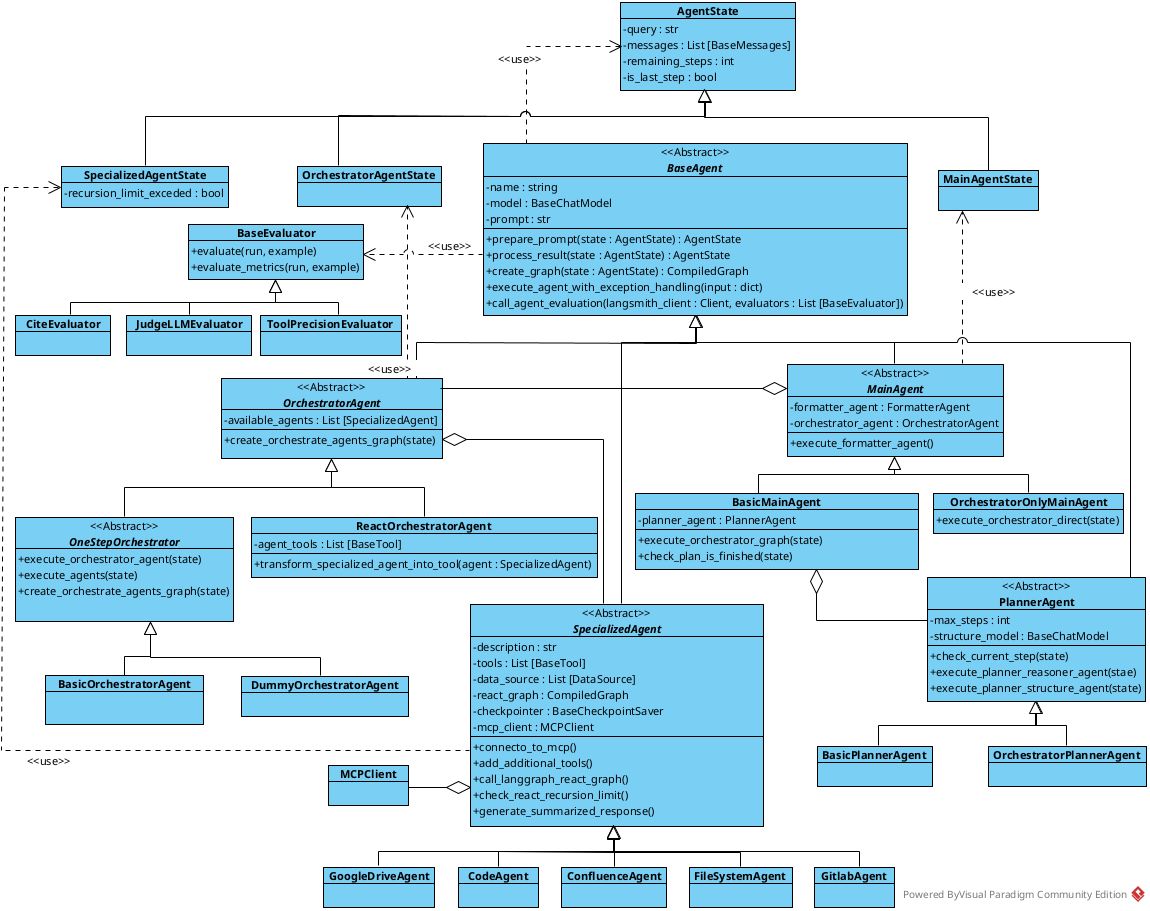
\includegraphics[width=1.4\linewidth]{figures/agentes.png}}
  \caption{Diagrama de clases UML de del sistema de agentes.}
  \label{fig:uml}
\end{figure}

El funcionamiento específico de cada tipo de agente se detalla en la Sección \ref{sec:diagrama_agentes}.

\section{Arquitectura del sistema}
El sistema implementado explora arquitecturas aplicables a entornos con restricciones de procesamiento, orientándose a responder consultas mediante el acceso eficiente a múltiples fuentes de datos. El diseño contempla las siguientes restricciones:
\begin{itemize}
\item\textbf{Ventana de contexto limitada: }los proyectos en producción pueden contener millones de líneas de código y documentación de comparable magnitud. Los modelos del estado del arte no poseen todavía la capacidad para procesar dicho volumen textual.
\item\textbf{Costo asociado: }incluso cuando el texto cabe en la ventana de contexto, las iteraciones con grandes volúmenes textuales generan un gasto computacional prohibitivo en entornos productivos. Esto crea la necesidad de optimizar selectivamente el acceso a la información.
\end{itemize}
Para abordar estas limitaciones, el sistema adopta un enfoque distribuido ilustrado en la Figura \ref{fig:agentes}. La arquitectura reparte el procesamiento entre agentes especializados, cada uno interactuando exclusivamente con su fuente asignada.
Estos agentes procesan los documentos originales y sintetizan únicamente la información pertinente, evitando así que niveles superiores deban procesar detalles irrelevantes. El agente orquestador analiza una operación y determina qué especialistas deben intervenir según las fuentes más apropiadas.
\begin{figure}[h]
\centering
\adjustbox{center=\textwidth}{\hspace{-1.2cm}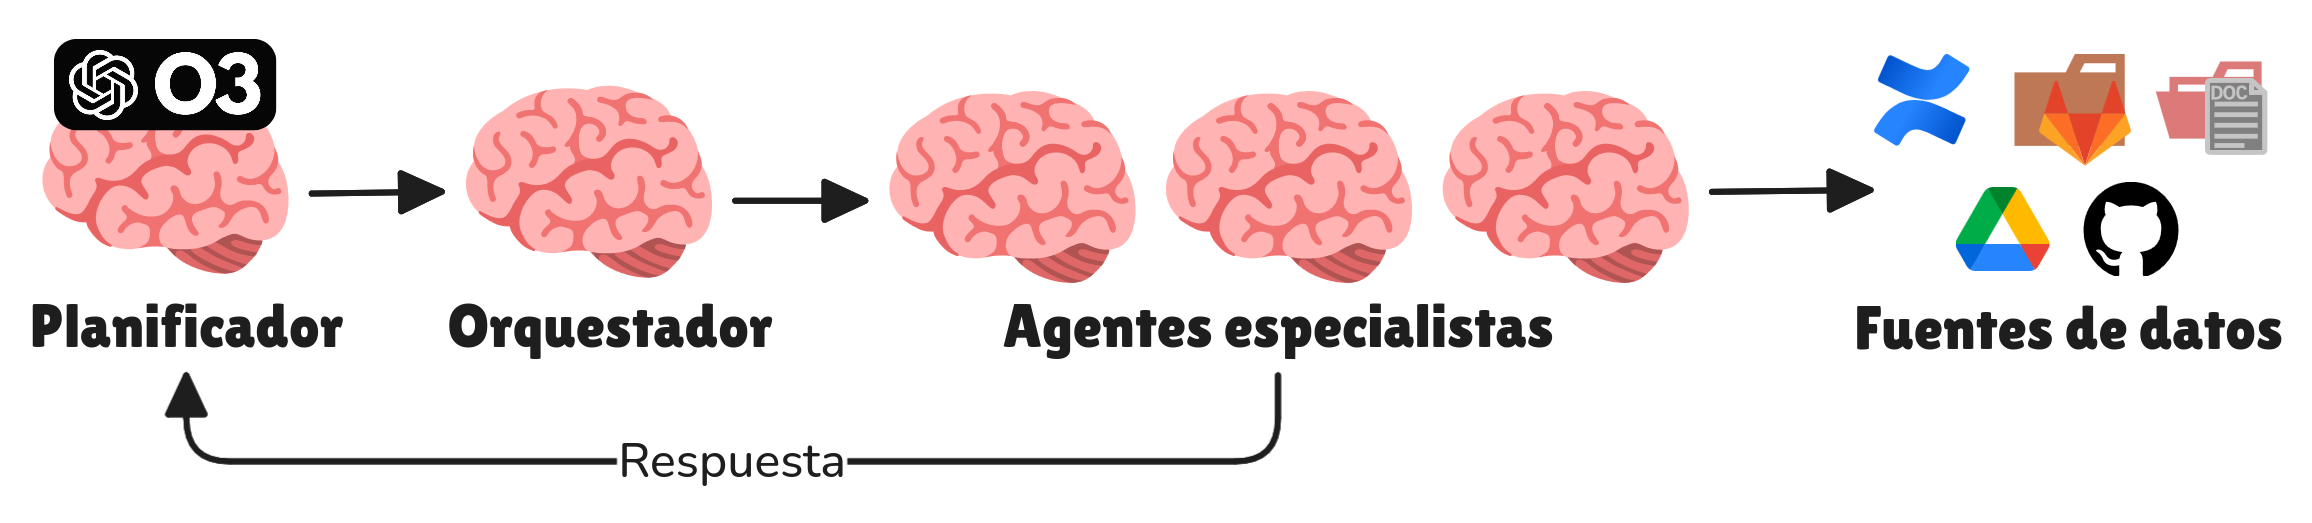
\includegraphics[width=1\linewidth]{figures/design.png}}
\caption{Esquema general de agentes del sistema}
\label{fig:agentes}
\end{figure}

Adicionalmente, se implementa una coordinación de alto nivel mediante el agente planificador, que establece la secuencia lógica de operaciones. Por ejemplo, ante una consulta sobre ejemplos de aplicación de la guía de estilos, se priorizaría localizar dicha guía para posteriormente examinar implementaciones específicas en el código fuente.

Una vez explicado el funcionamiento general del sistema; el Capítulo \ref{ch:chap7} explica en mayor profundidad cada variación implementada.

\subsection{Diagrama de agentes}
\label{sec:diagrama_agentes}

Como se puede observar en el diagrama de clases (Figura \ref{fig:uml}), la clase abstracta \opus{BaseAgent} constituye la base de la que heredan todos los agentes. Dicha clase establece las funcionalidades comunes que implementan todos los agentes del sistema:

\begin{itemize}
\item \textbf{Lógica de ejecución:} la función \opus{execute_agent_with_exception_handling()} se encarga de invocar el grafo definido en la función \opus{create_graph()}, gestionando las posibles excepciones e inicializando los parámetros de entrada requeridos. Todos los agentes derivados deben implementar la función \opus{prepare_prompt()} e integrarla en su grafo de ejecución correspondiente, para definir el mensaje inicial del sistema que instruye al agente.
\item \textbf{Gestión del resultado:} la función \opus{process_result()} se encarga de procesar y devolver el resultado de ejecución del agente para un estado específico. Este resultado varía según el agente; en los agentes especialistas corresponde a la respuesta que sintetiza su ejecución completa.
\item \textbf{Evaluación del agente:} la función \opus{call_agent_evaluation()} establece la lógica de evaluación específica para cada agente, utilizando las métricas definidas y representadas por la clase \opus{BaseEvaluator}. El Capítulo \ref{ch:chap9} describe este proceso en detalle.
\end{itemize}

Los agentes que heredan del agente base son los siguientes:
\begin{itemize}
  \item \textbf{SpecializedAgent:} representa de forma abstracta los agentes que realizan búsquedas en fuentes de información especializadas, aspecto detallado en el Capítulo \ref{ch:chap6}. Integra la lógica de gestión de las herramientas utilizadas mediante la clase \opus{MCPClient}, explicada en la Sección \ref{sec:gestionmcp}. Asimismo, contiene una secuencia de instancias de \opus{DataSource}, las cuales definen todos los documentos citables en las fuentes de datos disponibles, descrita en la Sección \ref{sec:citas}.
  \item \textbf{OrchestratorAgent:} implementa la lógica de enrutamiento de los agentes especialistas, determinando en cada caso qué agentes ejecutar para resolver una cuestión específica. Véase la Sección \ref{sec:agente_orquestador}.
  \item \textbf{PlannerAgent:} define la estrategia de planificación a seguir para una consulta determinada, elaborando planes secuenciales dinámicamente adaptables. Este proceso se detalla en la Sección \ref{sec:agente_planificador}.
  \item \textbf{FormatterAgent:} transforma una secuencia de ejecución de agentes en un resultado estructurado y comprensible, compuesto por una respuesta en formato textual y un conjunto de citas que referencian a documentos del proyecto software. 
  \item \textbf{MainAgent:} establece el flujo general de la ejecución, especificando si se implementarán agentes planificadores, orquestadores y enlazando su respuesta al agente formateador. Este proceso se describe en la Sección \ref{sec:principal}.
\end{itemize}

Cada agente implementa su propia clase de estado para gestionar los atributos vinculados a una ejecución específica. Estas clases extienden el estado común \opus{AgentState}, que incorpora atributos como los mensajes a incluir en el contexto de entrada. Como se ha descrito en la Sección \ref{sec:abst}, la interacción con los agentes sigue una estructura conversacional. Para materializar este enfoque, se utiliza la implementación de mensajes de LangChain: \opus{SystemMessage} para las directrices que instruyen al agente, \opus{HumanMessage} para las consultas o mensajes del usuario, y \opus{AIMessage} para incorporar las respuestas de otros agentes.

Durante la fase de inicialización, se procede a la creación de los grafos correspondientes a todos los agentes mediante la instanciación de sus respectivas clases, estableciendo simultáneamente las conexiones necesarias con los servidores MCP. Una vez completado este proceso de inicialización, los agentes adquieren la capacidad de responder a todas las consultas requeridas sin necesidad de reconexión. 

\section{Servidores MCP utilizados}
En esta sección se describirán los cinco servidores MCP utilizados, los cuales exponen sus herramientas mediante los dos protocolos de comunicación introducidos en la Sección \ref{sec:mcp_prots}: el protocolo SSE (Server-Sent Events) y el protocolo STDIO (Standard Input/Output).

\subsection{Servidores SSE}
Estos se alojan en componentes separados, ya que el protocolo SSE permite desacoplar servidores y cliente MCP.

\begin{itemize}
  \item \textbf{Servidor Confluence:} proporciona acceso de lectura al repositorio Confluence, utilizando el servidor MCP oficial de Atlassian\footnote{Repositorio de servidor MCP Atlassian: \url{https://github.com/sooperset/mcp-atlassian}}. El componente \opus{servidor_mcp_confluence} incorpora un script de lanzamiento \opus{launch_mcp_server_confluence.py} (detallado en el Listado \ref{lst:servconf}).

    El script inicializa el servidor mediante el gestor de paquetes uv, implementando el paquete mcp-atlassian\footnote{Paquete mcp-atlassian: \url{https://pypi.org/project/mcp-atlassian/}}. Este paquete integra el SDK de MCP para crear un servidor ASGI que maneja herramientas conectadas a la API de Atlassian. Tras la extracción de variables de entorno desde \opus{.env}, se ejecuta el comando uvx en el sistema.
    \begin{lstlisting}[caption={\protect\opus{launch_mcp_server_confluence.py}: ejecución de lanzamiento del servidor MCP Confluence},label={lst:servconf}]
    load_dotenv() 
    confluence_url = os.getenv('CONFLUENCE_URL')
    ...

    # Construir el comando para uvx
    command = ["uvx", "mcp-atlassian"]
    
    command.extend(["--transport", mcp_transport])
    command.extend(["--port", mcp_port]) 
    command.extend(["--confluence-url", confluence_url])
    command.extend(["--confluence-username", confluence_username])
    command.extend(["--confluence-token", confluence_token])

    # Ejecutar el comando
    try:
        subprocess.run(command)
    ...
\end{lstlisting}

\item\textbf{Servidor Código: }proporciona acceso de lectura al repositorio software, implementando herramientas para la consulta de su código fuente. Su desarrollo se ha realizado directamente mediante el SDK de MCP para Python\footnote{SDK de MCP para Python: \url{https://github.com/modelcontextprotocol/python-sdk}}, localizado en el fichero \opus{src/mcp_code_server.py} del componente \opus{servidor_mcp_bd_codigo}. La Sección \ref{sec:herramientas_codigo} detalla la implementación de dichas herramientas.

  El sistema emplea la clase \texttt{FastMCP}, que integra internamente un servidor ASGI para gestionar el enrutamiento de las herramientas implementadas. Como se especifica en el Listado \ref{lst:mcpcod}, el procedimiento consta de la instanciación de la clase, la asociación de diversas herramientas mediante el decorador \opus{mcp.tool}, y la posterior ejecución del servidor. Una vez vinculadas las herramientas, se generan automáticamente las rutas \opus{call_tool} y \opus{get_tools}, facilitando su acceso automatizado desde el cliente MCP.

\begin{lstlisting}[caption={\protect\opus{mcp_code_server.py:} ejecución del servidor MCP con acceso al código fuente},label={lst:mcpcod}]
  mcp = FastMCP("code_server_id")

  # Vincular herramientas al servidor
  @mcp.tool()
  async def get_all_respository_files_list() -> TextContent:
      """
      Devuelve una lista en formato string serializable a JSON de todos los ficheros en el repositorio respecto a su ruta relativa
      """
      files_list = get_all_files_list(db_session=db_session)
      files_list_str=str(files_list)
      return TextContent(
          text=files_list_str,
          type='text'
      )

  # Ejecutar servidor
  if __name__ == "__main__":
      try:
          mcp.run(transport='sse')
       ...

\end{lstlisting}


\end{itemize}

\subsection{Servidores STDIO}
\label{sec:stdio}
Estos servidores se ejecutan estableciendo una conexión en el cliente MCP mediante una instancia de \opus{StdioServerParameters}, que especifica los parámetros de configuración necesarios. De esta manera, cuando el cliente inicia la conexión, el servidor se ejecuta en un subproceso del mismo.

La configuración de dicha instancia sigue en los tres servidores el mismo procedimiento ilustrado en el Listado \ref{lst:mcpgitlab}. Se construye el comando con los argumentos correspondientes y se incorporan las credenciales como variables de entorno.

\begin{lstlisting}[caption={\protect\opus{mcp_multi_client.py}: instanciado de StdioServerParameters para el servidor MCP de GitLab},label={lst:mcpgitlab}]
  server_command = "npx"
  server_args = ["-y", "@modelcontextprotocol/server-gitlab"]

  # Obtener las credenciales desde las variables de entorno
  server_env = {
      "GITLAB_PERSONAL_ACCESS_TOKEN": os.getenv('GITLAB_PERSONAL_ACCESS_TOKEN'),
      "GITLAB_API_URL": GITLAB_API_URL
  }

  # Crear instancia StdioServerParameters indicando las credenciales de GitLab como variables de entorno para el servidor
  server_params = StdioServerParameters(
      command=server_command,
      args=server_args,
      env=server_env
  )
  
\end{lstlisting}
Mediante este procedimiento, se han utilizado los siguientes servidores:
\begin{itemize}
  \item\textbf{Servidor Sistema de ficheros local: }proporciona acceso a un directorio específico, que simula el repositorio de la ``documentación oficial'' del proyecto. Se ha utilizado el servidor de Anthropic FileSystem\footnote{FileSystem: \url{https://github.com/modelcontextprotocol/servers/tree/main/src/filesystem}}, ejecutándolo mediante el comando npx con el paquete del registro npm\footnote{Npm: \url{https://www.npmjs.com/}} \opus{@modelcontextprotocol/server-filesystem}\footnote{Server-filesystem: \url{https://www.npmjs.com/package/@modelcontextprotocol/server-filesystem}}.

  \label{sec:gitlab_mcp}
  \item\textbf{Servidor GitLab: }facilita el acceso al repositorio de GitLab con funcionalidades para leer o modificar ficheros, incidencias, usuarios y contribuciones. Se ejecuta utilizando el paquete npm \opus{@modelcontextprotocol/server-gitlab}\footnote{Server-gitlab: \url{https://www.npmjs.com/package/@modelcontextprotocol/server-gitlab}}. Debido a que no ofrece capacidades específicas para la lectura de ciertos recursos, se han desarrollado herramientas complementarias accediendo manualmente a la API de GitLab, detalladas en la Sección \ref{sec:agente_gitlab}.

\item\textbf{Servidor Google Drive: }proporciona acceso a un directorio de Google Drive, donde se alojan las maquetas HTML del proyecto software. A pesar de existir un repositorio oficial de MCP para la conexión con Google Drive, este no ofrece todas las funcionalidades requeridas, por lo que se ha empleado una modificación desarrollada en JavaScript\footnote{Servidor MCP Google Drive: \url{https://github.com/felores/gdrive-mcp-server/blob/main/index.ts}}. En consecuencia, en lugar de especificar el paquete a utilizar en la instancia \opus{StdioServerParameters}, se indica la ruta del script a ejecutar. También se ha modificado la herramienta de listar ficheros para mostrar recursivamente todos los ficheros dentro de los directorios listados.

Para obtener acceso al directorio de Google Drive mediante la API, se ha configurado una aplicación en Google Cloud\footnote{Google Cloud: \url{https://cloud.google.com/?hl=es}} siguiendo las directrices establecidas en el servidor MCP de Google Drive oficial\footnote{Directrices de autenticación: \url{https://github.com/modelcontextprotocol/servers/tree/main/src/gdrive}}. En dicha plataforma, se han obtenido las credenciales de acceso, las cuales se encuentran almacenadas en \opus{mcp_google_drive/credentials/gcp-oauth.keys.json}.

La API requiere de autenticación mediante el protocolo OAuth2.0\footnote{OAuth2.0: \url{https://oauth.net/2/}} con la cuenta de Google. Para la generación del token temporal \opus{.gdrive-server-credentials.json}, es necesario ejecutar el script del servidor especificando el parámetro auth, el cual iniciará el proceso de autenticación en el navegador.

\end{itemize}

\section{Cliente MCP}
\label{sec:gestionmcp}
Una vez explicada la estructura general de agentes y servidores MCP, en esta sección se detallará el mecanismo de comunicación entre los agentes y sus respectivos servidores para acceder a las herramientas disponibles.

Se ha implementado un cliente MCP mediante el patrón Singleton que permite gestionar todas las conexiones activas con los servidores MCP. Esta clase mantiene un diccionario para todas las herramientas y sesiones de conexiones MCP, utilizando el identificador del servidor como clave, tal como se ilustra en el Listado \ref{lst:mcpclient}.


\begin{lstlisting}[caption={\protect\opus{mcp_multi_client.py}: clase Singleton MCPClient},label={lst:mcpclient}]
  class MCPClient:
      _instance = None

      # Sesiones con servidores: id de servidor -> objeto de session
      _sessions: Dict[str, ClientSession] = {}
      # Herramientas disponibles por cada servidor: id servidor -> lista herramientas
      _tools: Dict[str, List[BaseTool]] = {}
      # Herramientas requeridas por cada agente: id agente -> nombre herramienta
      _agent_tools: Dict[str, List[str]] = {}
\end{lstlisting}

Para acceder a las herramientas, cada agente ejecuta los tres pasos secuenciales ilustrados en el Listado \ref{lst:mcpconnectgd}:

\begin{lstlisting}[caption={\protect\opus{google_drive_agent_graph.py}: función \protect\opus{connect_to_mcp} en agente Google Drive},label={lst:mcpconnectgd}]
  async def connect_to_mcp(self):
      # 1. Obtener instancia del cliente
      self.mcp_client = MCPClient.get_instance()
      # 2. Conectar al servidor correspondiente al agente  
      await self.mcp_client.connect_to_google_drive_server()
      # 3. Registrar agente y obtener herramientas
      self.mcp_client.register_agent(self.name, self.tools_str)
      self.tools = self.mcp_client.get_agent_tools(self.name)
\end{lstlisting}

La función de conexión al servidor correspondiente ejecutará la función del protocolo utilizado: \opus{connect_to_stdio_server()} (Listado \ref{lst:mcpstdio}) para STDIO y \opus{connect_to_sse_server()} (Listado \ref{lst:mcpsse}) para SSE.

\begin{lstlisting}[caption={\protect\opus{mcp_multi_client.py}: función \protect\opus{connect_to_stdio_server} en el cliente MCP},label={lst:mcpstdio}]
    async def connect_to_stdio_server(self, server_id: str, stdio_params: StdioServerParameters):
        # Establecer la conexión usando el exit_stack global
        stdio_transport = await global_exit_stack.enter_async_context(stdio_client(stdio_params))
        stdio, write = stdio_transport

        # Crear la sesión
        session = await global_exit_stack.enter_async_context(ClientSession(stdio, write))
        self._sessions[server_id] = session

        await self._initialize_session_and_load_tools(server_id)
\end{lstlisting}

\begin{lstlisting}[caption={\protect\opus{mcp_multi_client.py}: función \protect\opus{connect_to_sse_server} en el cliente MCP},label={lst:mcpsse}]
    async def connect_to_sse_server(self, server_id: str, host_ip: str, host_port: int):
        # Usar el exit_stack global
        streams = await global_exit_stack.enter_async_context(
            sse_client(f"http://{host_ip}:{host_port}/sse")
        )

        session = await global_exit_stack.enter_async_context(
            ClientSession(streams[0], streams[1])
        )
        self._sessions[server_id] = session

        await self._initialize_session_and_load_tools(server_id)
\end{lstlisting}

Las conexiones implementan el SDK de MCP, generando objetos \opus{ClientSession} en un \opus{AsyncExitStack} global. Esta pila gestiona la liberación automática de recursos y permite cerrar todas las conexiones de forma controlada mediante \opus{cleanup()}, como se detalla en el Listado \ref{lst:clean}.

\begin{lstlisting}[caption={\protect\opus{mcp_multi_client.py}: función \protect\opus{cleanup()} en el cliente MCP},label={lst:clean}]
    @staticmethod
    async def cleanup():
        try:
            if global_exit_stack:
                await global_exit_stack.aclose()
        ...

\end{lstlisting}

Finalmente, ambos protocolos ejecutan \opus{_initialize_session_and_load_tools()} (Listado \ref{lst:mcpinit}), que realiza tres tareas: inicializa la sesión de conexión, adapta las herramientas MCP a instancias \opus{BaseTool} de LangChain, y añade manejo de excepciones para evitar que los errores se propaguen al agente.

\begin{lstlisting}[caption={\protect\opus{mcp_multi_client.py}: función \protect\opus{_initialize_session_and_load_tools} en el cliente MCP},label={lst:mcpinit}]
  async def _initialize_session_and_load_tools(self, server_id: str):
    await self._sessions[server_id].initialize()
    # Adaptar herramientas a BaseTool de LangChain
    tools = await load_mcp_tools(self._sessions[server_id])
    # Añadir control de excepciones a las herramientas
    wrapped_tools = [patch_tool_with_exception_handling(tool) for tool in tools]
    self._tools[server_id] = wrapped_tools
\end{lstlisting}

\section{Estructura del proyecto}
El repositorio se estructura en cuatro componentes independientes, cada uno con su propio entorno virtual de Python, como ilustra la Figura \ref{fig:dir_principales}. El componente principal \opus{sistema_agentes} contiene todos los agentes desarrollados y el cliente MCP, organizando el código fuente en \opus{src}, los prompts y documentación en \opus{static}, las variables de configuración en \opus{config.py} y \opus{.env}, y la lógica principal en \opus{main.py}.

Los tres componentes restantes (\opus{servidor_mcp_bd_codigo}, \opus{servidor_mcp_confluence} y \opus{servidor_mcp_google_drive}) contienen cada uno un servidor MCP independiente.

\begin{figure}[p]
\centering
\definecolor{folderbg}{RGB}{124,166,198}
\definecolor{folderborder}{RGB}{110,144,169}
\newlength\Size
\setlength\Size{4pt}
\tikzset{%
  folder/.pic={%
    \filldraw [draw=folderborder, top color=folderbg!50, bottom color=folderbg] (-1.05*\Size,0.2\Size+5pt) rectangle ++(.75*\Size,-0.2\Size-5pt);
    \filldraw [draw=folderborder, top color=folderbg!50, bottom color=folderbg] (-1.15*\Size,-\Size) rectangle (1.15*\Size,\Size);
  },
  file/.pic={%
    \filldraw [draw=folderborder, top color=folderbg!5, bottom color=folderbg!10] (-\Size,.4*\Size+5pt) coordinate (a) |- (\Size,-1.2*\Size) coordinate (b) -- ++(0,1.6*\Size) coordinate (c) -- ++(-5pt,5pt) coordinate (d) -- cycle (d) |- (c) ;
  },
}
\forestset{%
  declare autowrapped toks={pic me}{},
  declare boolean register={pic root},
  pic root=0,
  pic dir tree/.style={%
    for tree={%
      folder,
      font=\ttfamily,
      grow'=0,
      % Reducción del espaciado vertical entre nodos
      s sep=0.09cm,
      % Reducción del espaciado horizontal entre niveles
      l sep=0.8cm,
    },
    before typesetting nodes={%
      for tree={%
        edge label+/.option={pic me},
      },
      if pic root={
        tikz+={
          \pic at ([xshift=\Size].west) {folder};
        },
        align={l}
      }{},
    },
  },
  pic me set/.code n args=2{%
    \forestset{%
      #1/.style={%
        inner xsep=2\Size,
        pic me={pic {#2}},
      }
    }
  },
  pic me set={directory}{folder},
  pic me set={file}{file},
}
\begin{forest}
  pic dir tree,
  pic root,
  for tree={% folder icons by default; override using file for file icons
    directory,
  },
  [tfg\_agentes\_software
    [servidor\_mcp\_bd\_codigo
    [src
    [mcp\_code\_server.py, file]
    ]
    ]
    [servidor\_mcp\_confluence
    [launch\_mcp\_server\_confluence.py, file]
    ]
    [servidor\_mcp\_google\_drive
    [credentials]
    [index\_mod.js, file]
    ]
    [sistema\_agentes
    [src
    [db]
    [evaluators]
    [mcp\_client]
    [main\_agent
    [main\_graph.py, file]
    ]
    [formatter\_agent]
    [orchestrator\_agent]
    [planner\_agent]
    [specialized\_agents
    [citation\_tools]
    [confluence\_agent]
    [filesystem\_agent]
    [gitlab\_agent]
    [google\_drive\_agent]
    [SpecializedAgent.py, file]
    ]
    [BaseAgent.py, file]
    [structured\_output\_validator.py, file]
    [utils.py, file]
    ]
    [static
    [gen\_docs
    ]
    [agent\_descriptions.py, file]
    [prompts.py, file]
    ]
    [main.py, file]
    [config.py, file]
    [.env, file]
    ]
  ]
\end{forest}
\caption{Estructura de directorios principales del proyecto}
\label{fig:dir_principales}
\end{figure}
